%&latex
\documentclass[11pt]{asaproc}

\usepackage{graphicx}

\usepackage{times}
\usepackage{subfigure} 

% For citations
\usepackage{natbib}

% For algorithms
\usepackage{algorithm}
\usepackage{algorithmic}
\usepackage{amsfonts}
\usepackage{amstext}
\usepackage{amssymb}
\usepackage{amsmath}

% For links
\usepackage{hyperref}
\usepackage[anythingbreaks]{breakurl}
% to compile w/ correct hyperlinks: 
% latex -> bibtex -> latex -> latex -> dvi2ps -> ps2pdf

% Fixes weird hyperref and algorithmic behavior
\newcommand{\theHalgorithm}{\arabic{algorithm}}

\title{On the Art and Science of Machine Learning Explanations\\\vspace{5pt}\small{A Discussion with Practical Recommendations and a Use Case}}
\author{Patrick Hall\thanks{H2O.ai, Mountain View, CA}
}
\begin{document}

\maketitle
\centerline{\today}

\vspace{15pt}

\begin{abstract}

This text discusses several explanatory methods that go beyond the error measurements and plots 			traditionally used to assess machine learning models. Some of the methods are tools of the trade while others are rigorously derived and backed by long-standing theory. The methods, decision tree surrogate models, individual conditional expectation (ICE) plots, local interpretable model-agnostic explanations (LIME), partial dependence plots, and Shapley explanations, vary in terms of scope, fidelity, and suitable application domain.  Along with descriptions of these methods, this text presents real-world usage recommendations supported by a use case and in-depth software examples.

\begin{keywords}
Machine learning, interpretability, explanations, transparency, FATML, XAI.
\end{keywords}
\end{abstract}

\section{Introduction}

Interpretability of complex machine learning models is a multifaceted, complex, and still evolving subject. Others have defined key terms and put forward general motivations for better intepretability of machine learning models (and lamented a general lack of scientific rigor) \cite{been_kim1}, \cite{gilpin2018explaining}, \cite{guidotti2018survey}, \cite{lipton1}. This applied text side-steps some looming, unsetttled intellectual matters to present viable practical methods for explaining the mechanisms and outputs of predictive models, typically supervised decision tree ensembles, for users who need to explain their work today. 

Following Doshi-Velez and Kim, this discussion uses ``the ability to explain or to present in understandable terms to a human,'' as the definition of \textit{interpretable}. ``When you can no longer keep asking why,'' will serve as the working definition for a \textit{good explanation} of model mechanisms or predictions \cite{gilpin2018explaining}. 
	
\begin{figure}[htb]
	\begin{center}
		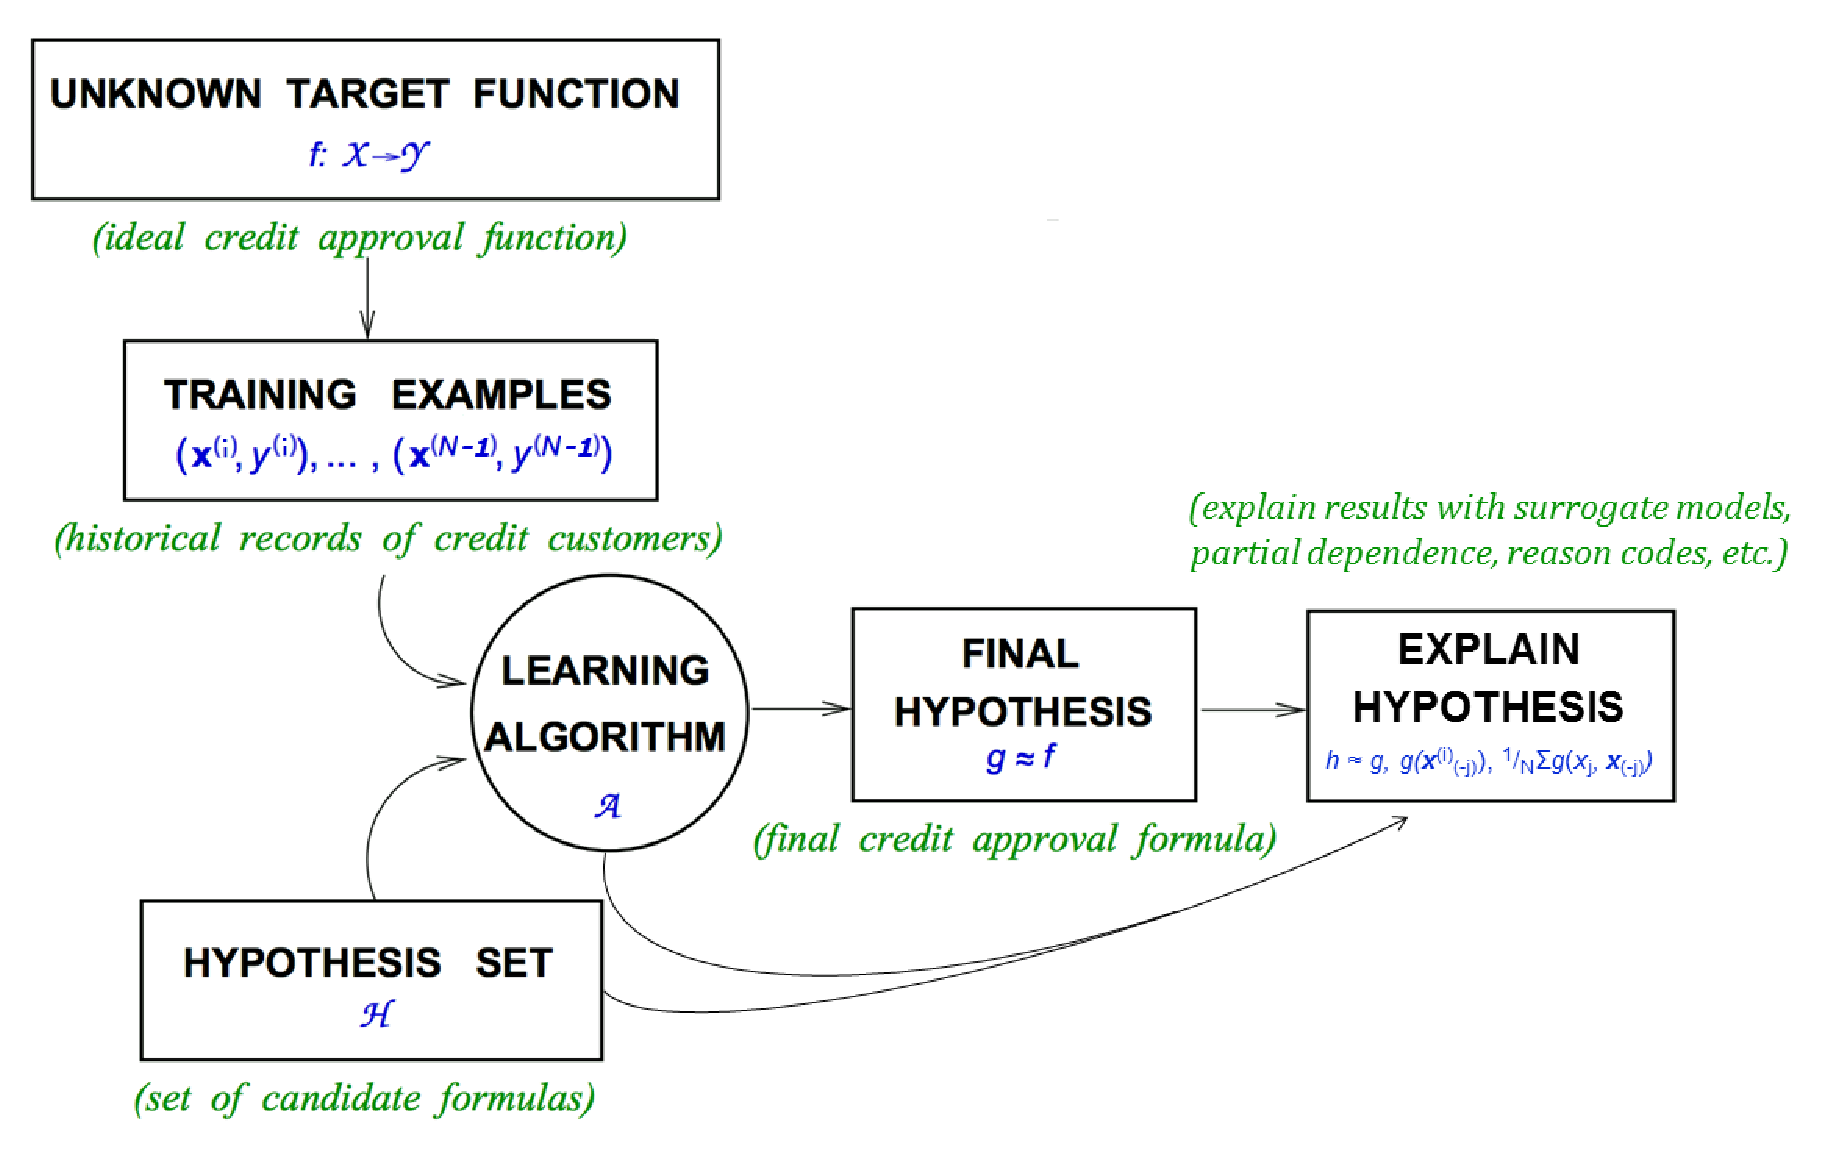
\includegraphics[scale=0.33]{img/figure_1.eps}
		\label{fig:learning_problem}
		\caption{An augmented learning problem diagram in which several techniques create explanations for a credit scoring model. Adapted from \textit{Learning From Data} \cite{lfd}.}
	\end{center}
\end{figure}	
	
As in Figure \ref{fig:learning_problem}, the presented explanatory methods help practitioners make random forests, GBMs, and other types of popular supervised  machine learning models more interpretable by enabling post-hoc explanations that are suitable for:\\

\begin{itemize}
	\item Facilitating regulatory compliance.
	\item Understanding or debugging model mechanisms and predictions.
	\item Preventing or debugging accidental or intentional discrimination by models.
	\item Preventing or debugging the malicious hacking or adversarial attack of models.
\end{itemize}

Detailed discussions of the explanatory methods begin below by defining notation. Then Sections \ref{sec:surrogate_dt} -- \ref{sec:shap} discuss explanatory methods and present recommendations for each method. Section \ref{sec:gen_rec} presents some general interpretability recommendations for practitioners. Section \ref{sec:use_case} applies some of the techniques and recommendations to the well-known UCI credit card dataset \cite{uci}. Section \ref{sec:suggested} discusses several additional interpretability subjects that are likely important for practitioners, and finally, Section \ref{sec:software} highlights software resources that accompany this text. 

%-------------------------------------------------------------------------------
\section{Notation} \label{sec:notation}
%-------------------------------------------------------------------------------

To facilitate technical descriptions of explanatory techniques, notation for input and output spaces, datasets, and models is defined.

\subsection{Spaces} 
 
	\begin{itemize}
		\item Input features come from the set $\mathcal{X}$ contained in a \textit{P}-dimensional input space,\\ $\mathcal{X} \subset \mathbb{R}^P$.  
		\item Known labels corresponding to instances of $\mathcal{X}$ come from the set $\mathcal{Y}$.
		\item Learned output responses come from the set $\mathcal{\hat{Y}}$. % For regression models, the set $\mathcal{\hat{Y}}_r$ is also contained in a $C$-dimensional output space, $\mathcal{\hat{Y}}_r \subset \mathbb{R}^{C_r}$. For classification models, the set $\mathcal{\hat{Y}}_c$ typically contains a column vector for each unique class in $\mathcal{Y}$. Hence, $\mathcal{\hat{Y}}_c$ is contained in a $C'$-dimensional output space,  $\mathcal{\hat{Y}}_c \subset \mathbb{R}^{C'_c}$.
	\end{itemize}	
	
\subsection{Datasets} 

	\begin{itemize}
		\item The input dataset $\mathbf{X}$ is composed of observed instances of the set $\mathcal{X}$ with a corresponding dataset of labels $\mathbf{Y}$, observed instances of the set $\mathcal{Y}$.
		\item Each $i$-th observation of $\mathbf{X}$ is denoted as $\mathbf{x}^{(i)} = $  
		$[x_0^{(i)}, x_1^{(i)}, \dots, x_{\textit{P}-1}^{(i)}]$, with corresponding $i$-th labels in $\mathbf{Y}, \mathbf{y}^{(i)}$, and corresponding predictions in $\mathbf{\hat{Y}}, \mathbf{\hat{y}}^{(i)}$. % = [y_0^{(i)}, y_1^{(i)}, \dots, y_{\textit{C}-1}^{(i)}]$.
		\item $\mathbf{X}$ and $\mathbf{Y}$ consists of $N$ tuples of observations: $[(\mathbf{x}^{(0)},\mathbf{y}^{(0)}), (\mathbf{x}^{(1)},\mathbf{y}^{(1)}), \dots,$\\$(\mathbf{x}^{(N-1)},\mathbf{y}^{(N-1)})]$. %\\ $\mathbf{x}^{(i)} \in \mathcal{X}$, $\mathbf{y}^{(i)} \in \mathcal{Y}$.
		\item Each $j$-th input column vector of $\mathbf{X}$ is denoted as $X_j = [x_{j}^{(0)}, x_{j}^{(1)}, \dots, x_{j}^{(N-1)}]^T$.
	\end{itemize}	 

\subsection{Models}

	\begin{itemize}
		\item A type of machine learning model $g$, selected from a hypothesis set $\mathcal{H}$, is trained to represent an unknown signal-generating function $f$ observed as  $\mathbf{X}$ with labels $\mathbf{Y}$ using a training algorithm $\mathcal{A}$: 
		$ \mathbf{X}, \mathbf{Y} \xrightarrow{\mathcal{A}} g$.
		\item $g$ generates learned output responses on the input dataset $g(\mathbf{X}) = \mathbf{\hat{Y}}$, and on the general input space $g(\mathcal{X}) = \mathcal{\hat{Y}}$.
		\item The model to be explained is denoted as $g$.
	\end{itemize}

%-------------------------------------------------------------------------------
\section{Surrogate Decision Trees} \label{sec:surrogate_dt}
%-------------------------------------------------------------------------------


The phrase \textit{surrogate model} is used here to refer to a simple model, $h$, of a complex model, $g$. This type of model is referred to by various other names, such as \textit{proxy} or \textit{shadow} models and the process of training surrogate models is sometimes referred to as \textit{model extraction} \cite{dt_surrogate1}, \cite{ff_interpretability},  \cite{dt_surrogate2}. 

\subsection{Description}

Given a learned function $g$, a set of learned output responses $g(\mathbf{X}) = \mathbf{\hat{Y}}$, and a tree splitting and pruning approach $\mathcal{A}$, a global -- or over all $\mathbf{X}$ -- surrogate decision tree $h_{\text{tree}}$ can be extracted such that $h_{\text{tree}}(\mathbf{X}) \approx g(\mathbf{X})$:

\begin{equation}
\mathbf{X}, g(\mathbf{X}) \xrightarrow{\mathcal{A}} h_{\text{tree}}
\end{equation}

Decision trees can be represented as directed graphs where the relative positions of input features can provide insight into their importance and interactions \cite{cart}. This makes decision trees useful surrogate models. Input features that appear high and often in the directed graph representation of $h_{\text{tree}}$ are assumed to have high importance in $g$. Input features directly above or below one-another in $h_{\text{tree}}$ are assumed to have potential interactions in $g$. These relative relationships between input features in $h_{\text{tree}}$ can be used to verify and analyze the feature importance, interactions, and predictions of $g$.

\begin{figure}
	\begin{center}
		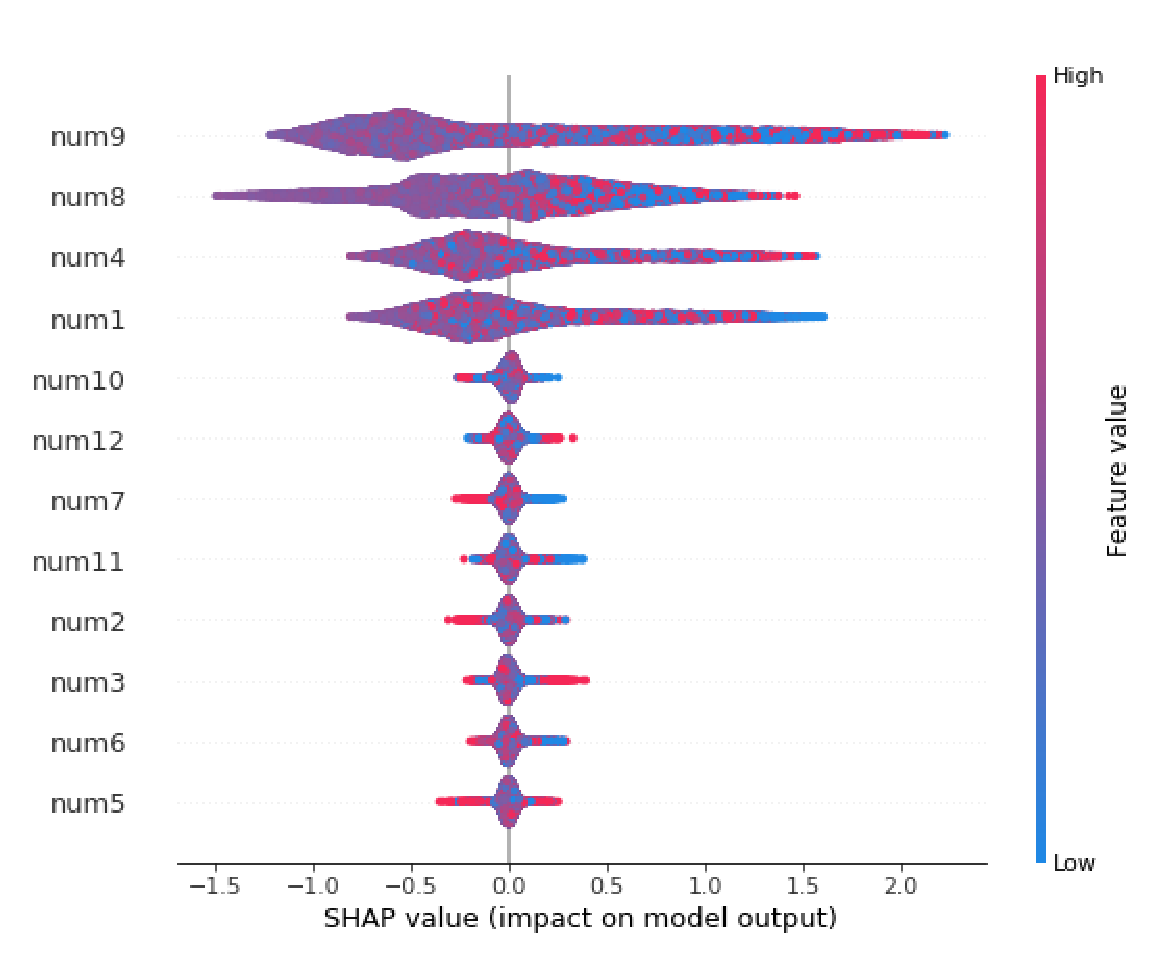
\includegraphics[scale=0.4]{img/figure_2.eps}
		\caption{Shapley summary plot for known signal-generating function $f = \text{num} _1 * \text{num}_4 + |\text{num}_8| * \text{num}_9^2 + e$, and for learned GBM response function $g_{\text{GBM}}$.}
		\label{fig:global_shapley}
	\end{center}
\end{figure}

Figures \ref{fig:global_shapley} and \ref{fig:dt_surrogate} use simulated data to empirically demonstrate the desired relationships between input feature importance and interactions in the input space $\mathbf{X}$, the label space $f(\mathbf{X}) = \mathbf{Y}$, a GBM model to be explained $g_{\text{GBM}}$, and a decision tree surrogate $h_{\text{tree}}$. Data with a known signal-generating function depending on four input features with interactions and with eight noise features is simulated such that: 

\begin{equation}
\label{eq:f}
f = \text{num} _1 * \text{num}_4 + |\text{num}_8| * \text{num}_9^2 + e
\end{equation}

\noindent$g_{\text{GBM}}$ is trained: $ \mathbf{X}, \mathbf{f(X)} \xrightarrow{\mathcal{A}} g_{\text{GBM}}$ such that $g_{\text{GBM}} \approx f$. Then $h_{\text{tree}}$ is extracted by $\mathbf{X}, g_{\text{GBM}}(\mathbf{X}) \xrightarrow{\mathcal{A}} h_{\text{tree}}$, such that $h_{\text{tree}}(\mathbf{X}) \approx g_{\text{GBM}}(\mathbf{X}) \approx f(\mathbf{X})$.

Figure \ref{fig:global_shapley} displays the local Shapley contribution values for an input feature's impact on each $g_{\text{GBM}}(\mathbf{X})$ prediction. Analyzing local Shapley values can be a more holistic and consistent feature importance metric than traditional single-value quantities \cite{shapley}. Features are ordered from top to bottom by their mean absolute Shapley value across observations in Figure \ref{fig:global_shapley}, and as expected, $\text{num}_9$ and $\text{num}_8$ tend to make the largest contributions to $g_{\text{GBM}}(\mathbf{X})$ followed by $\text{num}_4$ and $\text{num}_1$. Also as expected, noise features make minimal contributions to $g_{\text{GBM}}(\mathbf{X})$. Shapley values are discussed in detail in Section \ref{sec:shap}.

Figure \ref{fig:dt_surrogate} is a directed graph representation of $h_{\text{tree}}$ that prominently displays the importance of input features $\text{num}_9$ and $\text{num}_8$ along with $\text{num}_4$ and $\text{num}_1$. Figure \ref{fig:dt_surrogate} also visually highlights the potential interactions between these inputs. URLs to the data and software used to generate Figures \ref{fig:global_shapley} and \ref{fig:dt_surrogate} are available in Section \ref{sec:software}.

\begin{figure}[htb]
	\begin{center}
		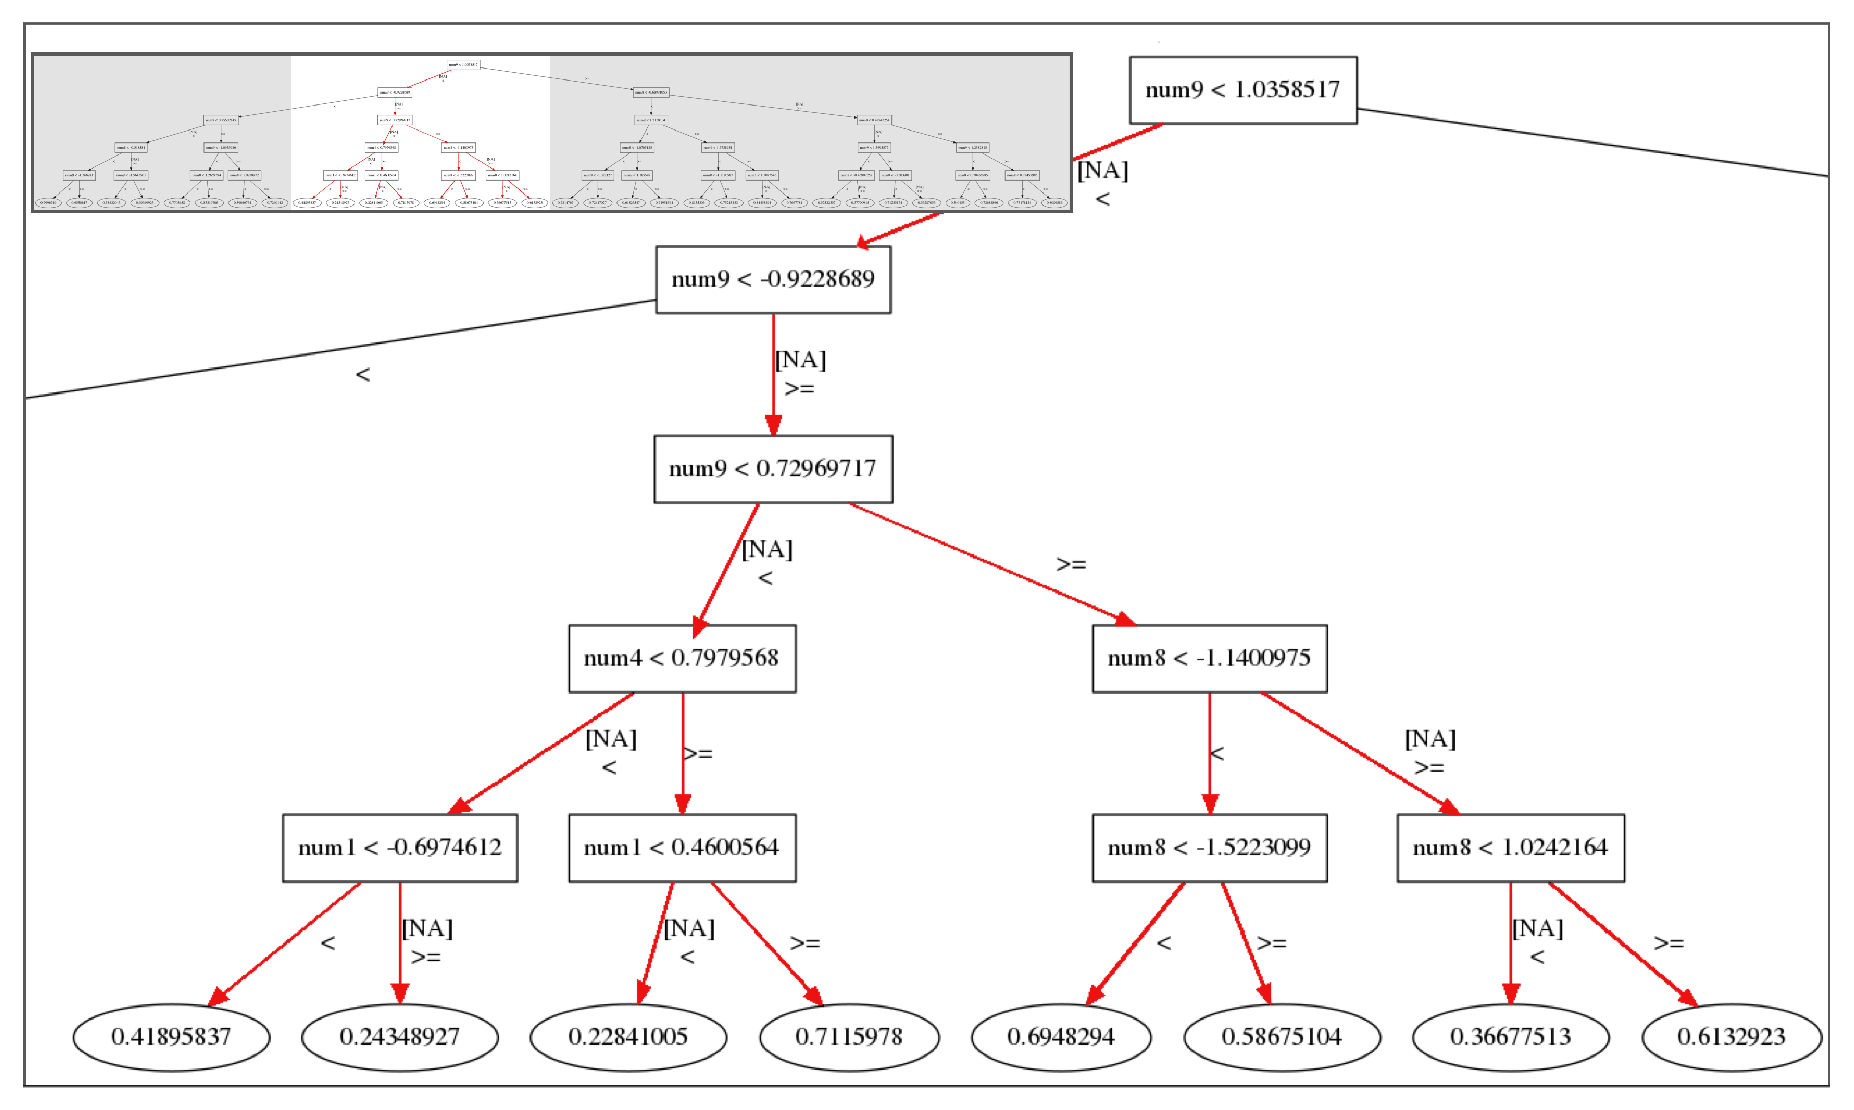
\includegraphics[scale=0.3]{img/figure_3.eps}
		\caption{$h_{\text{tree}}$ for previously defined known signal-generating function $f$ and learned GBM response function $g_{\text{GBM}}$. An image of the entire $h_{\text{tree}}$ directed graph is available in the supplementary materials described in Section \ref{sec:software}.}
		\label{fig:dt_surrogate}
	\end{center}
\end{figure}

\subsection{Recommendations}

\begin{itemize}
	
	\item A shallow-depth $h_{\text{tree}}$ displays a global, low-fidelity (e.g. approximate), high-interpretability flow chart of important features and interactions in $g$. Because there are few theoretical gaurantees that $h_{\text{tree}}$ truly represents $g$, always use error measures to assess the trustworthiness of $h_{\text{tree}}$.
	
	\item Prescribed methods for training $h_{\text{tree}}$ do exist \cite{dt_surrogate1} \cite{dt_surrogate2}. In practice, straightforward cross-validation approaches are often sufficient. Moreover, comparing cross-validated training error to traditional training error can give an indication of the stability of the single decision tree, $h_{\text{tree}}$.
	
	\item Hu et al. use local linear surrogate models, $h_{\text{GLM}}$, in $h_{\text{tree}}$ leaf nodes to increase overall surrogate model fidelity while also retaining a high degree of interpretability \cite{lime-sup}.
	
\end{itemize}

%-------------------------------------------------------------------------------
\section{Partial Dependence and Individual Conditional Expectation (ICE) plots}
\label{sec:pd_ice}
%-------------------------------------------------------------------------------

Partial dependence (PD) plots are a widely-used method for describing the average predictions of a complex model $g$ across some partition of data $\mathbf{X}$ for some interesting input feature $X_j$ \cite{esl}. Individual conditional expectation (ICE) plots are a newer method that describes the local behavior of $g$ for a single instance $\mathbf{x} \in \mathcal{X}$. Partial dependence and ICE can be combined in the same plot to identify interactions modeled by $g$ and to create a holistic portrait of the predictions of a complex model for some $X_j$  \cite{ice_plots}.

\subsection{Description}
	
Following Friedman et al. a single feature $X_j \in \mathbf{X}$ and its complement set $\mathbf{X}_{(-j)} \in \mathbf{X}$ (where $X_j \cup \mathbf{X}_{(-j)} = \mathbf{X}$) is considered. $\text{PD}(X_j, g)$ for a given feature $X_j$ is estimated as the average output of the learned function $g(\mathbf{X})$ when all the components of $X_j$ are set to a constant $x \in \mathcal{X}$ and $\mathbf{X}_{(-j)}$ is left unchanged. $\text{ICE}(x_j, \mathbf{x}, g)$ for a given instance $\mathbf{x}$ and feature $x_j$ is estimated as the output of $g(\mathbf{x})$ when $x_j$ is set to a constant $x \in \mathcal{X}$ and all other features $\mathbf{x} \in \mathbf{X}_{(-j)}$ are left untouched. Partial dependence and ICE curves are usually plotted over some set of constants $x \in \mathcal{X}$. 

\begin{figure}[htb]
	\begin{center}
		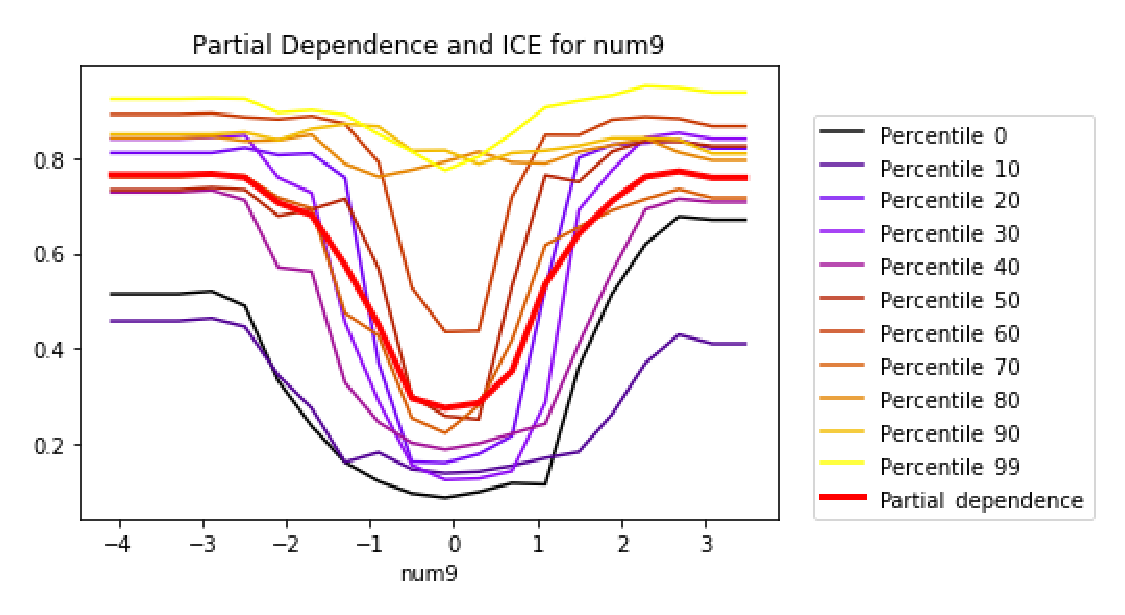
\includegraphics[scale=0.5]{img/figure_4.eps}
		\caption{Partial dependence and ICE curves for previously defined known signal-generating function $f$,  learned GBM response function $g_{\text{GBM}}$, and important input feature $\text{num}_9$.}
		\label{fig:pdp_ice}
	\end{center}
\end{figure}

As in Section \ref{sec:surrogate_dt}, simulated data is used to highlight desirable characteristics of partial dependence and ICE plots. In Figure \ref{fig:pdp_ice} partial dependence and ICE at the minimum, maximum, and each decile of $g_{\text{GBM}}(\mathbf{X})$ are plotted. The known quadratic behavior of $\text{num}_9$ is plainly visible, except for high value predictions, the 80\textsuperscript{th} percentiles of $g_{\text{GBM}}(\mathbf{X})$ and above and for $\sim-1 < \text{num}_9 < \sim1$. When partial dependence and ICE curves diverge, this often points to an interaction that is being averaged out of the partial dependence. Given the form of Equation \ref{eq:f}, there is a known interaction between $\text{num}_9$ and $\text{num}_8$. Combining the information from partial dependence and ICE plots with $h_{tree}$ can help elucidate more detailed information about modeled interactions in $g$. For the simulated example, $h_{tree}$ shows an interaction between $\text{num}_9$ and $\text{num}_8$ and additional modeled interactions between $\text{num}_9$, $\text{num}_4$, and $\text{num}_1$ for $\sim -0.92 \le \text{num}_9 <  \sim 1.04.$ URLs to the data and software used to generate Figure \ref{fig:pdp_ice} are available in Section \ref{sec:software}.

\subsection{Recommendations}

\begin{itemize}

\item Combining $h_{\text{tree}}$ with partial dependence and ICE curves is a convenient method for detecting, confirming, and understanding important interactions in $g$.

\item As monotonicity is often a desired trait for interpretable models, partial dependence and ICE plots can be used to verify the monotonicity of $g$ on average and across percentiles of $g(\mathbf{X})$ w.r.t. some input feature $X_j$.

\end{itemize}

%-------------------------------------------------------------------------------
\section{Local Interpretable Model-agnostic Explanations (LIME)}
\label{sec:lime}
%-------------------------------------------------------------------------------

Global and local scope are key concepts in explaining machine learning models and predictions. Section \ref{sec:surrogate_dt} presents decision trees as a global -- or over all $\mathbf{X}$ -- surrogate model. As learned response functions, $g$, can be complex, simple global surrogate models can sometimes be too approximate to be trustworthy. LIME attempts to create more representative explanations by fitting a local surrogate model, $h$, in the local region of some observation of interest $\mathbf{x} \in \mathcal{X}$. Both $h$ and local regions can be defined to suit the needs of users.

\subsection{Description}

Ribeiro et al. specifies LIME for some observation $\mathbf{x} \in \mathcal{X}$ as:

\begin{equation}
\begin{aligned}
\underset{h \in \mathcal{H}}{\arg\min}\:\mathcal{L}(g, h, \pi_{\mathbf{X}}) + \Omega(h)
\end{aligned}
\end{equation}

\noindent where $h$ is an interpretable surrogate model of $g$, often a linear model $h_{GLM}$, $\pi_{\mathbf{X}}$ is a weighting function over the domain of $g$, and $\Omega(h)$ limits the complexity of $h$ \cite{lime}. Following Ribeiro et al. $h_{GLM}$ is often trained by:

\begin{equation}
\begin{aligned}
\mathbf{X}', g(\mathbf{X}') \xrightarrow{\mathcal{A}_{\text{LASSO}}} h_{\text{GLM}}
\end{aligned}
\end{equation}

\noindent where $\mathbf{X}'$ is sampled from $\mathcal{X}$, $\pi_{\mathbf{X}}$ weighs $\mathbf{X}'$ samples by their Euclidean similarity to $\mathbf{x}$ to enforce locality, local feature contributions are estimated as the product of $h_{\text{GLM}}$ coefficients and their associated observed values $\beta_j x_j$, and $\Omega(h)$ is defined as a LASSO, or L1, penalty on $h_{\text{GLM}}$ coefficients inducing sparsity in $h_{GLM}$. 		

Figure \ref{fig:lime} displays estimated local feature contribution values for the same $g_{\text{GBM}}$ and simulated $\mathbf{X}$ with known signal-generating function $f$ used in previous sections. To increase the nonlinear capacity of the three $h_{GLM}$ models, information from the Shapley summary plot in Figure \ref{fig:global_shapley} is used to select inputs to discretize before training each $h_{GLM}$: $\text{num}_1, \text{num}_4, \text{num}_8$ and $\text{num}_9$. Table \ref{tab:lime} contains prediction and fit information for $g_{\text{GBM}}$ and $h_{\text{GLM}}$. This is critical information for analyzing LIMEs.

\begin{table}[ht]
	\centering
	\caption{$g_{\text{GBM}}$ and $h_{GLM}$ predictions and $h_{GLM}$ intercepts and fit measurements for the $h_{GLM}$ models trained to explain $g_{\text{GBM}}(\mathbf{x}^{(i)})$ at the 10\textsuperscript{th}, median, and 90\textsuperscript{th} percentiles of previously defined $g_{\text{GBM}}(\mathbf{X})$ and known signal-generating function $f$.} 
	%\tiny
	\begin{tabular}{ | p{1.7cm} | p{1.7cm} | p{1.7cm} | p{1.5cm}| p{1cm} | }
	\hline
	$g_{\text{GBM}}(\mathbf{X})$ Percentile & $g_{\text{GBM}}(\mathbf{x})$ Prediction & $h_{GLM}(\mathbf{x})$ Prediction & $h_{GLM}$ Intercept & $h_{GLM}$ R\textsuperscript{2} \\ 
	\hline
	10\textsuperscript{th} & 0.16 & 0.13 & 0.53 & 0.72\\
	\hline	
	Median & 0.30 & 0.47 & 0.70 & 0.57\\
	\hline	
	90\textsuperscript{th} & 0.82 & 0.86 & 0.76 & 0.40\\
	\hline
	\end{tabular}
	\label{tab:lime}
\end{table}	

\begin{figure*}[htb]
	\begin{center}
		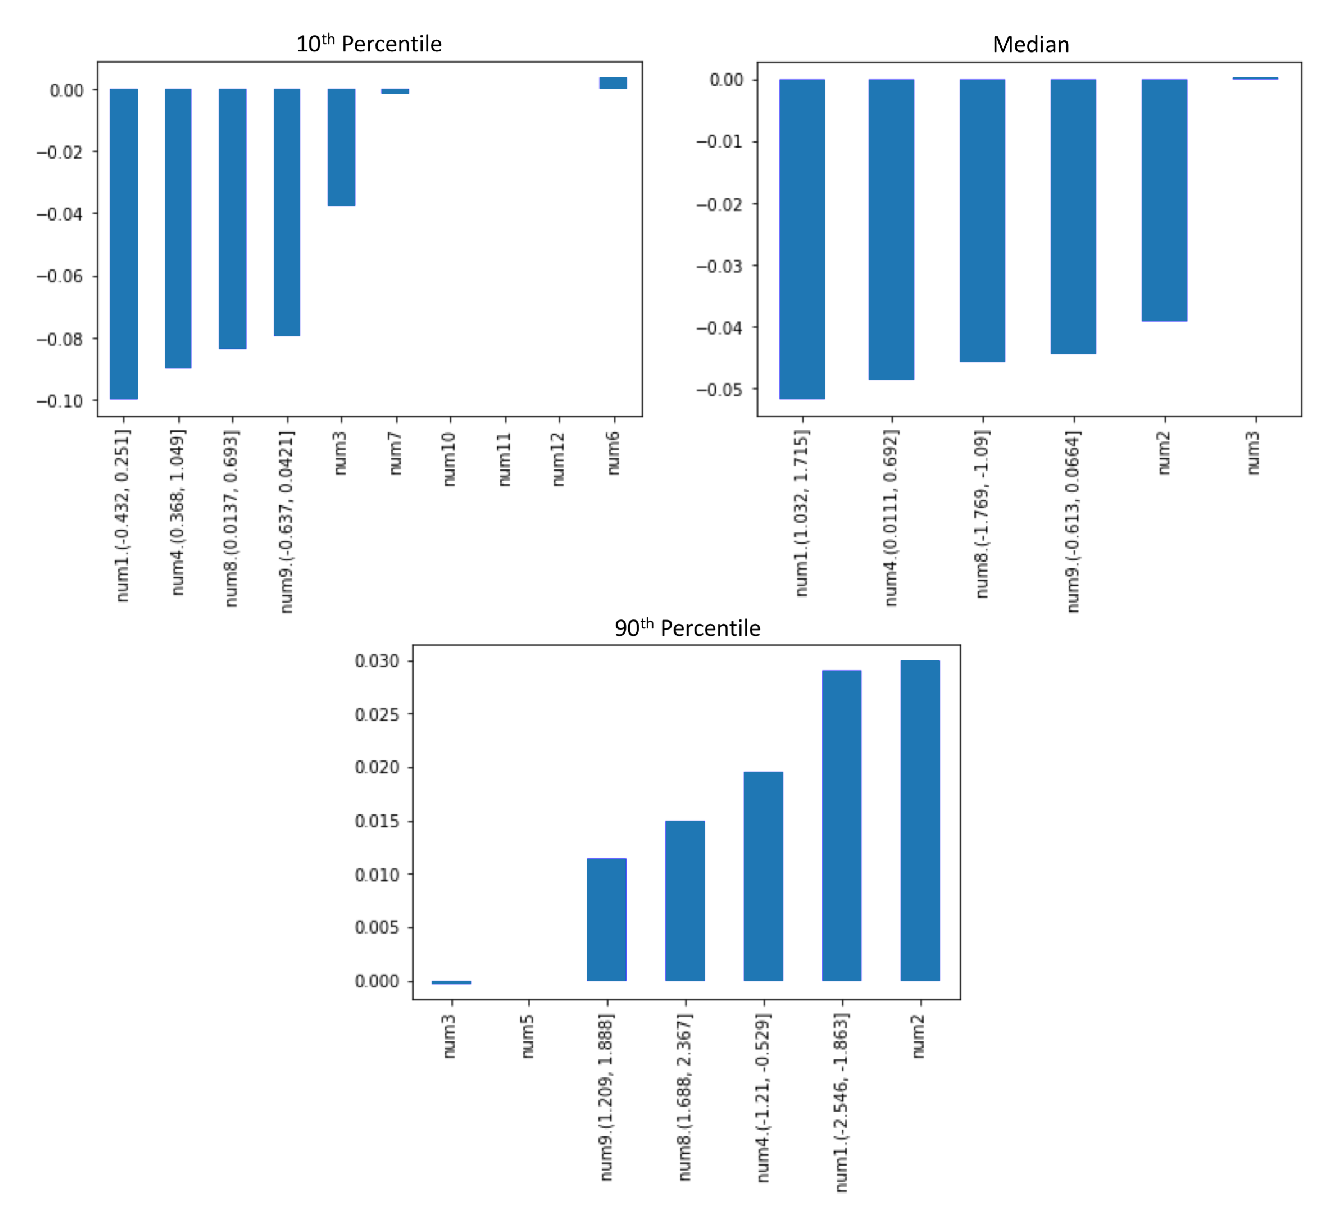
\includegraphics[scale=0.6]{img/figure_5.eps}
		\caption{Sparse, low-fidelity local feature contributions found using LIME at three percentiles of $g_{\text{GBM}}(\mathbf{X})$ for known signal-generating function $f = \text{num} _1 * \text{num}_4 + |\text{num}_8| * \text{num}_9^2 + e$.}
		\label{fig:lime}
	\end{center}
\end{figure*}

Table \ref{tab:lime} shows that LIME is not necessarily locally accurate, meaning that the predictions of $h_{GLM}(\mathbf{x})$ are not always equal to the prediction of $g_{\text{GBM}}(\mathbf{x})$. Moreover, the three $h_{GLM}$ models do not necessarily explain all of the variance of $g_{\text{GBM}}$ predictions in the local regions around the three $\mathbf{x}^{(i)}$ of interest. $h_{GLM}$ intercepts are also displayed because local feature contribution values, $\beta_j x_j^{(i)}$, are offsets from the local $h_{GLM}$ intercepts.

An immediately noticeable characteristic of the estimated local contributions in Figure \ref{fig:lime} is their sparsity. LASSO input feature selection drives some $h_{GLM}$ $\beta_j$ coefficients to zero so that some $\beta_j x_j^{(i)}$ local feature contributions are also zero. For the 10\textsuperscript{th} percentile $g_{\text{GBM}}(\mathbf{X})$ prediction, the local $h_{GLM}$ R\textsuperscript{2} is adequate and the LIME values appear parsimonious with reasonable expectations. The contributions from discretized $\text{num}_1, \text{num}_4, \text{num}_8$ and $\text{num}_9$ outweigh all other noise feature contributions and the $\text{num}_1, \text{num}_4, \text{num}_8$ and $\text{num}_9$ contributions are all negative, as expected for the relatively low value of $g_{\text{GBM}}(\mathbf{x})$. 

For the median prediction of $g_{\text{GBM}}(\mathbf{X})$, it could be expected that some estimated contributions for $\text{num}_1, \text{num}_4, \text{num}_8$ and $\text{num}_9$ should be positive and others should be negative. However, all local feature contributions are negative due to the relatively high value of the $h_{\text{GLM}}$ intercept at the median percentile of $g_{\text{GBM}}(\mathbf{X})$. Because the $h_{\text{GLM}}$ intercept is quite large compared to the $g_{\text{GBM}}(\mathbf{x}^{(i)})$ prediction, it is not alarming that all the $\text{num}_1, \text{num}_4, \text{num}_8$ and $\text{num}_9$ contributions are negative offsets w.r.t. the local $h_{GLM}$ intercept value. For the median $g_{\text{GBM}}(\mathbf{X})$ prediction, $h_{\text{GLM}}$ also estimates that the noise feature $\text{num}_2$ has a fairly large contribution and the local $h_{GLM}$ R\textsuperscript{2} is probably less than adequate to generate fully trustworthy explanations.

For the 90\textsuperscript{th} percentile of $g_{\text{GBM}}(\mathbf{X})$ predictions, the local contributions for $\text{num}_1, \text{num}_4, \text{num}_8$ and $\text{num}_9$ are positive as expected for the relatively high value of $g_{\text{GBM}}(\mathbf{x^{(i)}})$, but the local $h_{GLM}$ R\textsuperscript{2} is somewhat poor and the noise feature $num2$ has the highest local feature contribtion. This large attribution to the noise feature $\text{num}2$ could stem from problems in the LIME procedure or in the fit of $g_{\text{GBM}}$ to $f$. Further investigation, or model debugging, is conducted in Section \ref{sec:shap}.

Generally the LIMEs in Section \ref{sec:lime} would be considered to be sparse or high-interpretability but also low-fidelity explanations. This is not always the case with LIME and the fit of some $h_{GLM}$ to a local region around some $g(\mathbf{x})$ will vary in accuracy. URLs to the data and software used to generate Table \ref{tab:lime} and Figure \ref{fig:lime} are available in Section \ref{sec:software}.

\subsection{Recommendations}

\begin{itemize}
	
	\item Always use fit measures to assess the trustworthiness of LIMEs.

	\item Local feature contribution values are often offsets from a local $h_{GLM}$ intercept. Note that this intercept can sometimes account for the most important local phenomena. Each LIME feature contribution can be interpreted as the difference in $h(\mathbf{x})$ and some local offset, often $\beta_0$, associated with some  feature $x_j$.

	\item Some LIME methods can be difficult to deploy for explaining predictions in real-time. Consider highly deployable variants for real-time applications \cite{h2o_mli_booklet}, \cite{lime-sup}.
		
	\item Always investigate local $h_{GLM}$ intercept values. Generated LIME samples can contain large proportions of out-of-domain data that can lead to unrealistic intercept values. 
		
	\item To increase the fidelity of LIMEs, try LIME on discretized input features and on manually constructed interactions. Use $h_{\text{tree}}$ to construct potential interaction terms.
 	
	\item Use cross-validation to estimate standard deviations or even confidence intervals for local feature contribution values.
	
	\item When relying only on local linear models, note that LIME can fail to create acceptable explanations, particularly in the presence of extreme nonlinearity or high-degree interactions. Other types of local models with model-specific explanatory mechanisms, such as decision trees or neural networks, can be used in these cases. 
	
\end{itemize}

%-------------------------------------------------------------------------------
\section{Tree Shap} \label{sec:shap}
%-------------------------------------------------------------------------------

Shapley explanations, including tree shap and even certain implementations of LIME, are a class of additive, consistent local feature contribution measures with long-standing theoretical support \cite{shapley}. Shapley explanations are the only possible locally accurate and consistent feature contribution values, meaning that Shapley explanation values for input features always sum to $g(\mathbf{x})$ and that Shapley explanation values can never decrease for some $x_j$ when $g$ is changed such that $x_j$ truly makes a stronger contribution to $g(\mathbf{x})$ \cite{shapley}. 

\vspace{10pt}

\subsection{Description}

For some observation $\mathbf{x} \in \mathcal{X}$, Shapley explanations take the form:

\begin{equation}
\label{eq:shap_additive}
\begin{aligned}
g(\mathbf{x}) = \phi_0 + \sum_{j=0}^{j=\mathcal{P} - 1} \phi_j \mathbf{z}_j
\end{aligned}
\end{equation}

\noindent In Equation \ref{eq:shap_additive}, $\mathbf{z} \in \{0,1\}^\mathcal{P}$ is a binary representation of $\mathbf{x}$ where 0 indicates missingness. Each $\phi_j$ is the local feature contribution value associated with $x_j$ and $\phi_0$ is the average of $g(\mathbf{X})$. 

Shapley values can be estimated in different ways. Tree shap is a specific implementation of Shapley explanations. It does not rely on surrogate models. Both tree shap and a related technique known as \textit{treeinterpreter} rely instead on traversing internal tree structures to estimate the impact of each $x_j$ for some $g(\mathbf{x})$ of interest \cite{tree_shap}, \cite{treeinterpreter}.

\begin{equation}
\label{eq:shap_contrib}
\begin{aligned}
\phi_{j} = \sum_{S \subseteq \mathcal{P} \setminus \{j\}}\frac{|S|!(\mathcal{P} -|S| -1)!}{\mathcal{P}!}[g_x(S \cup \{j\}) - g_x(S)]
\end{aligned}
\end{equation}

\noindent Unlike treeinterpreter and as displayed in Equation \ref{eq:shap_contrib}, tree shap and other Shapley approaches estimate $\phi_j$ as the difference between the model prediction on a subset of features $S$ without $X_j$, $g_x(S)$, and the model prediction with $X_j$ and $S$, $g_x(S \cup \{j\})$, summed and weighed appropriately across all subsets $S$ of $\mathcal{P}$ that do not contain $X_j$, $S \subseteq \mathcal{P} \setminus \{j\}$. (Here $g_x$ incorporates the mapping between $\mathbf{x}$ and the binary vector $\mathbf{z}$.) Since trained decision tree response functions model complex dependencies between input features, removing different subsets of input features helps elucidate the true impact of removing $x_j$ from $g(\mathbf{x})$.

\begin{figure*}[htb]
	\begin{center}
		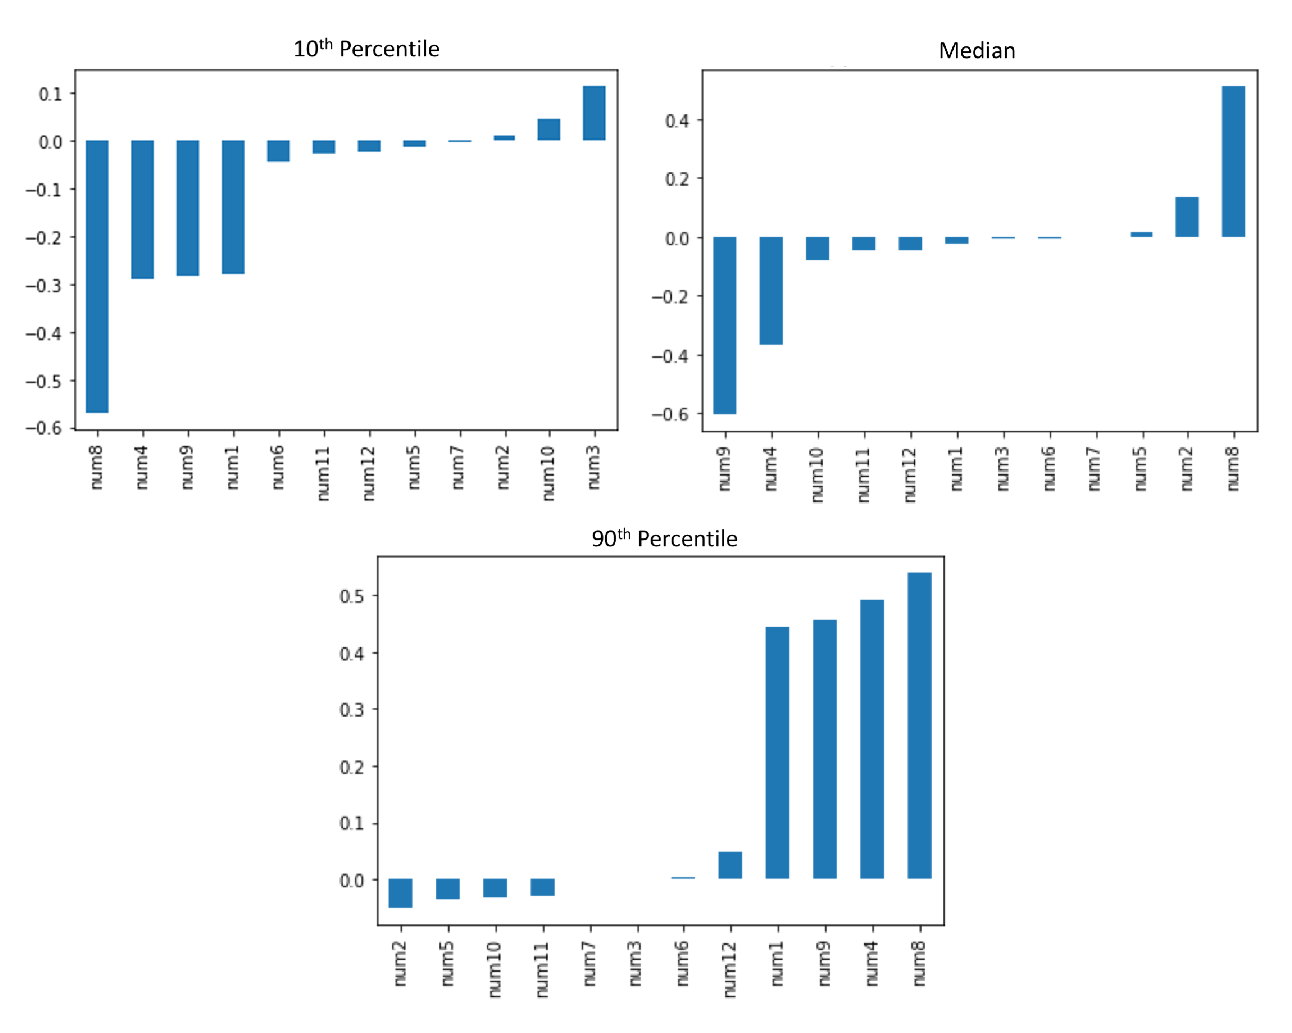
\includegraphics[scale=0.6]{img/figure_6.eps}
		\caption{Complete, consistent local feature contributions found using tree shap at three percentiles of $g_{\text{GBM}}(\mathbf{X})$ and for known signal generating function $f = \text{num} _1 * \text{num}_4 + |\text{num}_8| * \text{num}_9^2 + e$.}
		\label{fig:shap}
	\end{center}
\end{figure*}

Simulated data is used again to illustrate the utility of tree shap. Shapley explanations are estimated at the 10\textsuperscript{th}, median, and 90\textsuperscript{th} percentiles of $g_{\text{GBM}}(\mathbf{X})$ for simulated $\mathbf{X}$ with known signal-generating function $f$. Results are presented in Figure \ref{fig:shap}. In contrast to the LIME explanations in Figure \ref{fig:lime}, the Shapley explanations are complete, giving a numeric local contribution value for each non-missing input feature. At the 10\textsuperscript{th} percentile of $g_{\text{GBM}}(\mathbf{X})$ predictions, all feature contributions for $\text{num}_1, \text{num}_4, \text{num}_8$ and $\text{num}_9$ are negative as expected for this relatively low value of $g_{\text{GBM}}(\mathbf{X})$ and their contributions obviously outweigh those of noise features.

For the median prediction of $g_{\text{GBM}}(\mathbf{X})$, the Shapley explanations are somewhat aligned with the expectation of a split between positive and negative contributions. $\text{num}_1, \text{num}_4$, and $\text{num}_9$ are negative and the contribution for $\text{num}_8$ is positive. Like the LIME explanations at this percentile in Figure \ref{fig:lime}, the noise feature $\text{num}_2$ has a relatively high contribution, higher than that of $\text{num}_1$, likely indicating that $g_{\text{GBM}}$ is over-emphasizing $\text{num}_2$ in the local region around the median prediction. 

As expected at the 90\textsuperscript{th} percentile of $g_{\text{GBM}}(\mathbf{X})$ all contributions from $\text{num}_1, \text{num}_4, \text{num}_8$ and $\text{num}_9$ are positive and much larger than the contributions from noise features. Unlike the LIME explanations at the 90\textsuperscript{th} percentile of $g_{\text{GBM}}(\mathbf{X})$ in Figure \ref{fig:lime}, tree shap estimates only a small contribution from $\text{num}_2$. This discrepancy may reveal a pair-wise linear correlation between $\text{num}_2$ and $g_{\text{GBM}}(\mathbf{X})$ in the local region around the 90\textsuperscript{th} percentile of $g_{\text{GBM}}(\mathbf{X})$ that fails to represent the true form of $g_{\text{GBM}}(\mathbf{X})$ in this region, which can be highly nonlinear and incorporate high-degree interactions. Partial dependence and ICE for $\text{num}_2$ and two-dimensional partial dependence between $\text{num}_2$ and $\text{num}_1, \text{num}_4, \text{num}_8$ and $\text{num}_9$ could be used to further investigate the form of $g_{\text{GBM}}(\mathbf{X})$ w.r.t. $\text{num}_2$, along with model debugging techniques discussed briefly in Section \ref{sec:suggested}. URLs to the data and software used to generate Figure \ref{fig:shap} are available in Section \ref{sec:software}.

\subsection{Recommendations}

\begin{itemize}
	
	\item Tree shap is ideal for estimating high-fidelity, consistent, and complete explanations of decision tree and decision tree ensemble models, perhaps even in regulated applications to generate regulator-mandated reason codes (also known as turn-down codes or adverse action codes).
	
	\item Because tree shap explanations are offsets from a global intercept, each $\phi_j$ can be interpreted as the difference in $g(\mathbf{x})$ and the average of $g(\mathbf{X})$ associated with some input feature $x_j$ \cite{molnar}. 
		
	\item Currently treeinterpreter may be inappropriate for some GBM models. Treeinterpreter is locally accurate for some decision tree and random forest models, but is known to be inconsistent like all other feature importance methods aside from Shapley approaches \cite{tree_shap}. In experiments available in the supplemental materials of this text, treeinterpreter is seen to be locally inaccurate for some XGBoost GBM models. 
	
\end{itemize}

%-------------------------------------------------------------------------------
\section{General Recommendations} \label{sec:gen_rec}
%-------------------------------------------------------------------------------

The following recommendations apply to several or all of the described explanatory techniques or to the practice of applied interpretable machine learning in general.

\begin{itemize}	
	
	\item Less complex models are typically easier to explain. Section \ref{sec:suggested} contains information about directly interpretable white-box machine learning models.
	
	\item Monotonicity is often a desirable characteristic in interpretable models. White-box, monotonically constrained \href{https://github.com/dmlc/xgboost}{XGBoost} models along with the explanatory techniques described in this text are a direct and open source way to train and explain an interpretable machine learning model. A monotonically constrained XGBoost GBM is trained and explained in Section \ref{sec:use_case}.
	
	\item Several explanatory techniques are usually required to create good explanations for any given complex model. Users should apply a combination global and local and low- and high-fidelity explanatory techniques to a machine learning model and seek consistent results across multiple explanatory techniques. Simpler low-fidelity or sparse explanations can be used to understand more accurate, and sometimes more sophisticated, high-fidelity explanations.  

	\item Methods relying on surrogate models or generated data are sometimes unpalatable to users. Users sometimes \textit{need} to understand \textit{their} model on \textit{their} data.
	
	\item Surrogate models can provide low-fidelity explanations for an entire machine learning pipeline in the original feature space if $g$ is defined to include feature extraction or feature engineering steps.
	
	\item Both understanding and trust are crucial to interpretability. The discussed explanatory techniques should engender a greater understanding of model mechanisms and predictions. But can a model be trusted to perform as expected on unseen data? Its predictions probably do not extrapolate linearly outside of the training, validation, or test data domains. Always conduct sensitivity analysis on your trained machine learning model to understand how it will behave on out-of-domain data.
	
	\item Consider production deployment of explanatory methods carefully. Currently, the deployment of some open source software packages is not straightforward, especially for the generation of explanations on new data in real-time.
	
\end{itemize}

%-------------------------------------------------------------------------------
\section{Credit Card Data Use Case} \label{sec:use_case}
%-------------------------------------------------------------------------------

Some of the discussed explanatory techniques and recommendations will now be applied to a basic credit scoring problem using a monotonically constrained XGBoost binomial classifier and the UCI credit card dataset \cite{uci}. Referring back to Figure \ref{fig:learning_problem}, a training set $X$ and associated labels $Y$ will be used to train a GBM with decision tree base learners, selected based on domain knowledge from many other types of hypotheses models $\mathcal{H}$, using a monotonic splitting strategy with gradient boosting as the training algorithm $\mathcal{A}_{\text{mono}}$, to learn a final hypothesis model $g_{\text{mono}}$, that approximates the true signal generating function $f$ governing credit default in $\mathcal{X}$ and $\mathcal{Y}$ such that $g_{\text{mono}} \sim f$:

\begin{equation}
\label{eq:cc_training}
\begin{aligned}
\mathbf{X}, \mathbf{Y} \xrightarrow{\mathcal{A_{\text{mono}}}} g_{\text{mono}}
\end{aligned}
\end{equation}

\noindent$g_{\text{mono}}$ is globally explainable with aggregated local Shapley values, decision tree surrogate models $h_{\text{tree}}$, partial dependence, and ICE plots. Additionally each prediction made by $g_{\text{mono}}$ can be explained using local Shapley explanations. 

To begin, Pearson correlation between $g_{\text{mono}}$ inputs and the target, \texttt{default payment next month}, are calculated and stored. All other features except for the observation identifier, \texttt{ID}, are used as $g_{\text{mono}}$ inputs. Then 30\% of the credit card dataset observations are randomly partitioned into a labeled validation set. Pearson correlations are used to define monotonicity constraints w.r.t. each input feature. Input features with a positive correlation to the target are constrained to a monotonically increasing relationship with the target under $g_{\text{mono}}$. Input features with a negative correlation to the target are constrained to a monotonically decreasing relationship. Along with the monotonicity constraints, the non-default hyperparameter settings used to train $g_{\text{mono}}$ are presented in Table \ref{tab:mono_gbm}. 

\begin{table}[ht]
	\centering
	\caption{$g_{\text{mono}}$ hyperparameters for the UCI credit card dataset. Adequate hyperparameters were found by Cartesian grid search.}
	%\tiny
	\begin{tabular}{ | p{3.5cm} | p{1.2cm} | }
	\hline
	Hyperparameter & Value \\ 
	\hline
	\texttt{eta} & 0.08 \\
	\hline	
	\texttt{subsample} & 0.9 \\
	\hline	
	\texttt{colsample\_bytree} & 0.9 \\
	\hline
	\texttt{maxdepth} & 15 \\	
	\hline
	\end{tabular}
	\label{tab:mono_gbm}
\end{table}	 

\noindent A maximum of 1000 iterations were used to train $g_{\text{mono}}$, with early stopping triggered after 50 iterations without validation AUC improvement. This configuration led to a final validation AUC of 0.781 after only 100 iterations. 

\begin{figure*}[htb]
	\begin{center}
		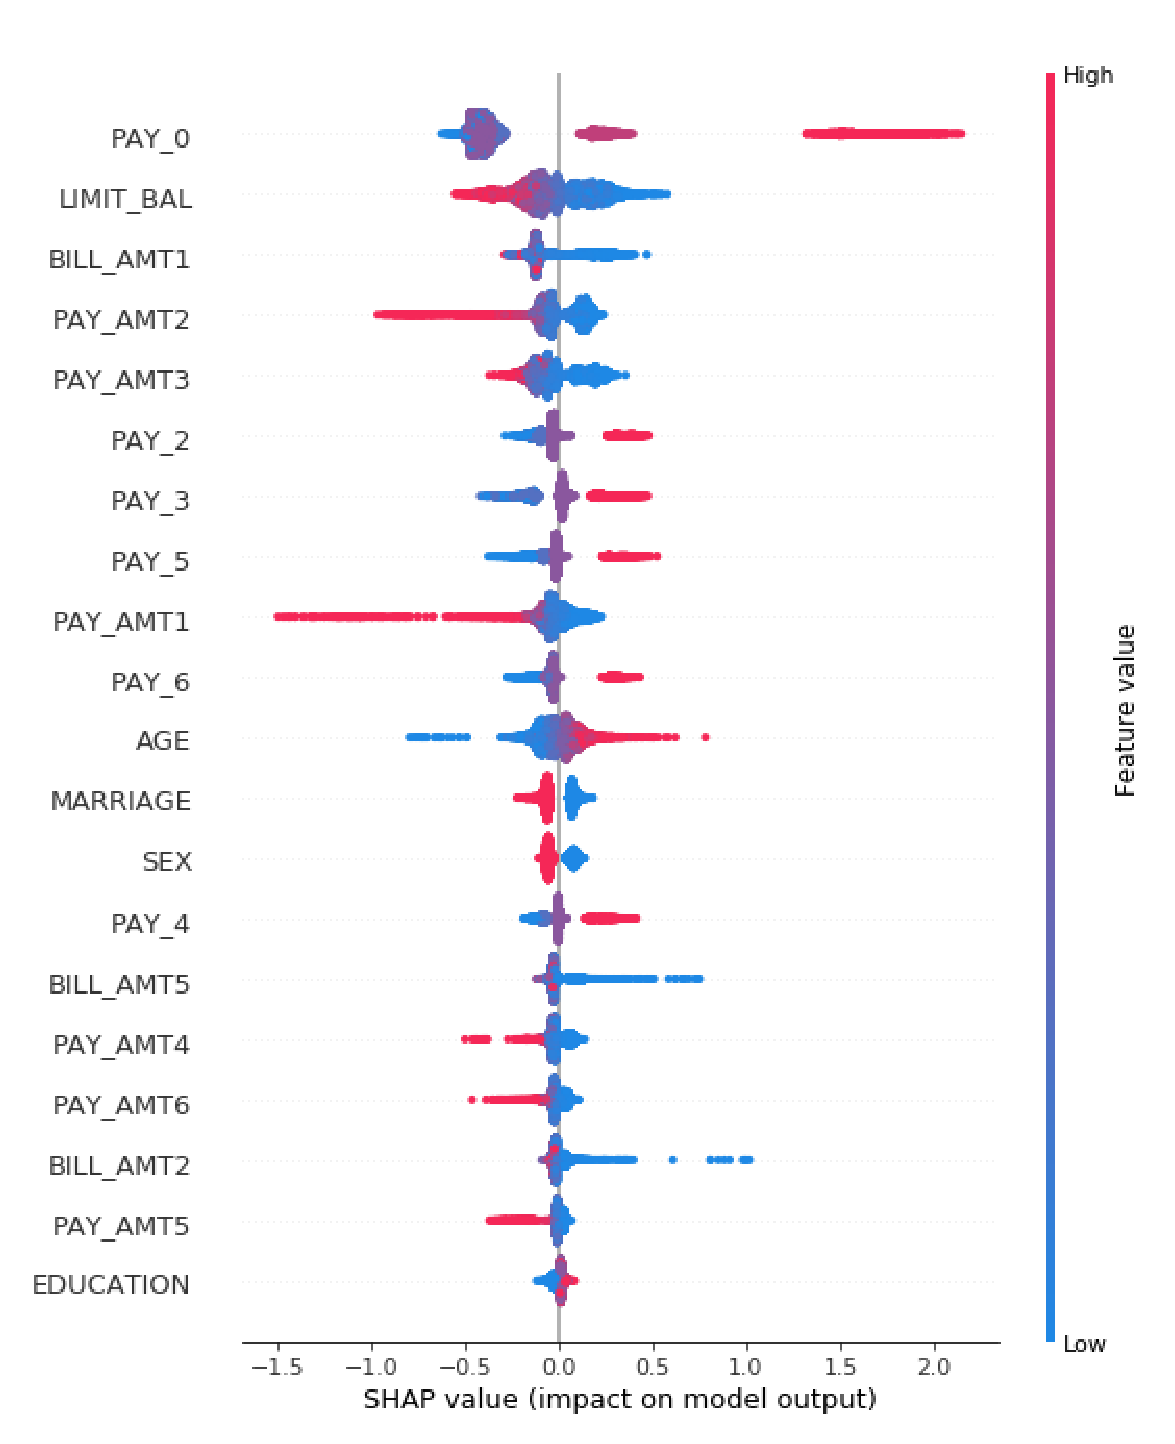
\includegraphics[scale=0.4]{img/figure_7.eps}
		\caption{Shapley summary plot for $g_{\text{mono}}$ in a 30\% validation set randomly sampled from the UCI credit card dataset.}
		\label{fig:cc_global_shapley}
	\end{center}
\end{figure*}

The global feature importance of $g_{\text{mono}}$ evaluated in the validation set and ranked by mean absolute Shapley value is displayed in Figure \ref{fig:cc_global_shapley}. \texttt{PAY\_0} -- a customer's most recent repayment status, \texttt{LIMIT\_BAL} -- a customer's credit limit, and \texttt{BILL\_AMT1} -- a customer's most recent bill amount are the globally most important features, which aligns with reasonable expectations and basic domain knowledge. (A real-world credit scoring application would be unlikely to use \texttt{LIMIT\_BAL} as an input feature because this feature could cause target leakage. \texttt{LIMIT\_BAL} is used in this small data example to improve $g_{\text{mono}}$ fit.) The monotonic relationship between each input feature and $g_{\text{mono}}$ output is also visible in Figure \ref{fig:cc_global_shapley}. Numeric Shapley explanation values appear to increase only as an input feature value increases as for \texttt{PAY\_0}, or vice versa, say for \texttt{LIMIT\_BAL}. 

\begin{figure*}[htb]
	\begin{center}
		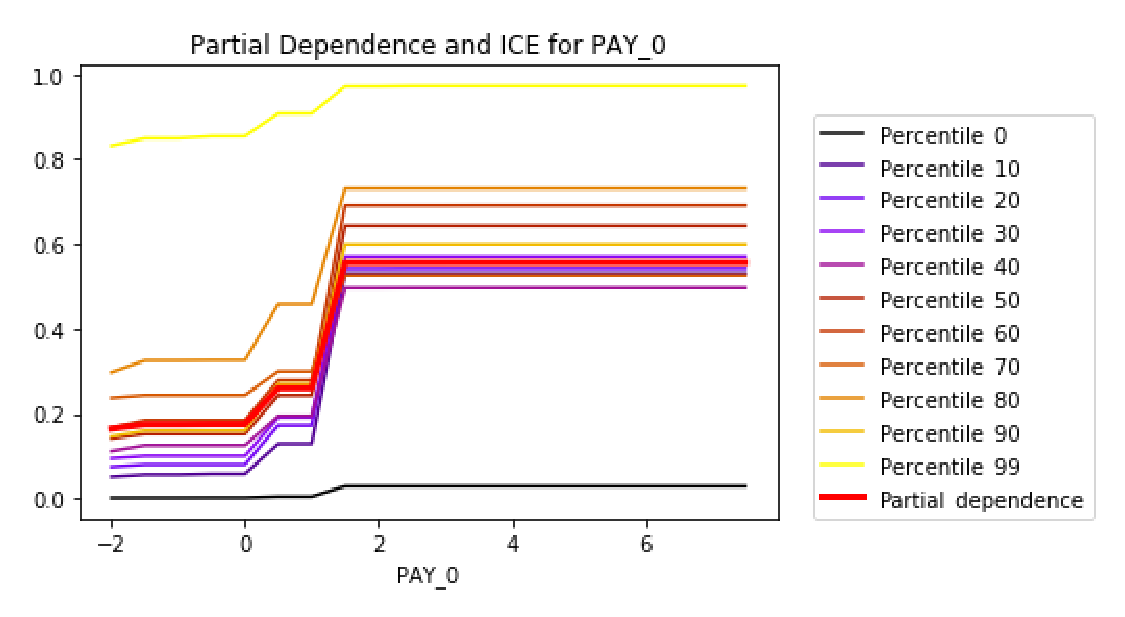
\includegraphics[scale=0.6]{img/figure_8.eps}
		\caption{Partial dependence and ICE curves for learned GBM response function $g_{\text{mono}}$, and important input feature $\text{PAY\_0}$.}
		\label{fig:cc_pdp_ice}
	\end{center}
\end{figure*}

Partial dependence and ICE for $g_{\text{mono}}$ and the important input feature \texttt{PAY\_0} verify the monotonic increasing behavior of $g_{\text{mono}}$ w.r.t. to \texttt{PAY\_0}. For several percentiles of predicted probabilities and on average, the output of $g_{\text{mono}}$ is low for \texttt{PAY\_0} values -2 -- 1 then increases dramatically. \texttt{PAY\_0} values of -2 -- 1 are associated with on-time or 1 month late payments. A large increase in predicted probability of default occurs at \texttt{PAY\_0 = 2} and predicted probabilities plateau after \texttt{PAY\_0 = 2}. The lowest and highest predicted probability customers do not display the same precipitous jump in predicted probability at \texttt{PAY\_0 = 2}. If this dissimilar prediction behavior is related to interactions with other input features, that may be evident in a surrogate decision tree model.

\vspace{10pt}

\begin{figure*}[htb]
	\begin{center}
		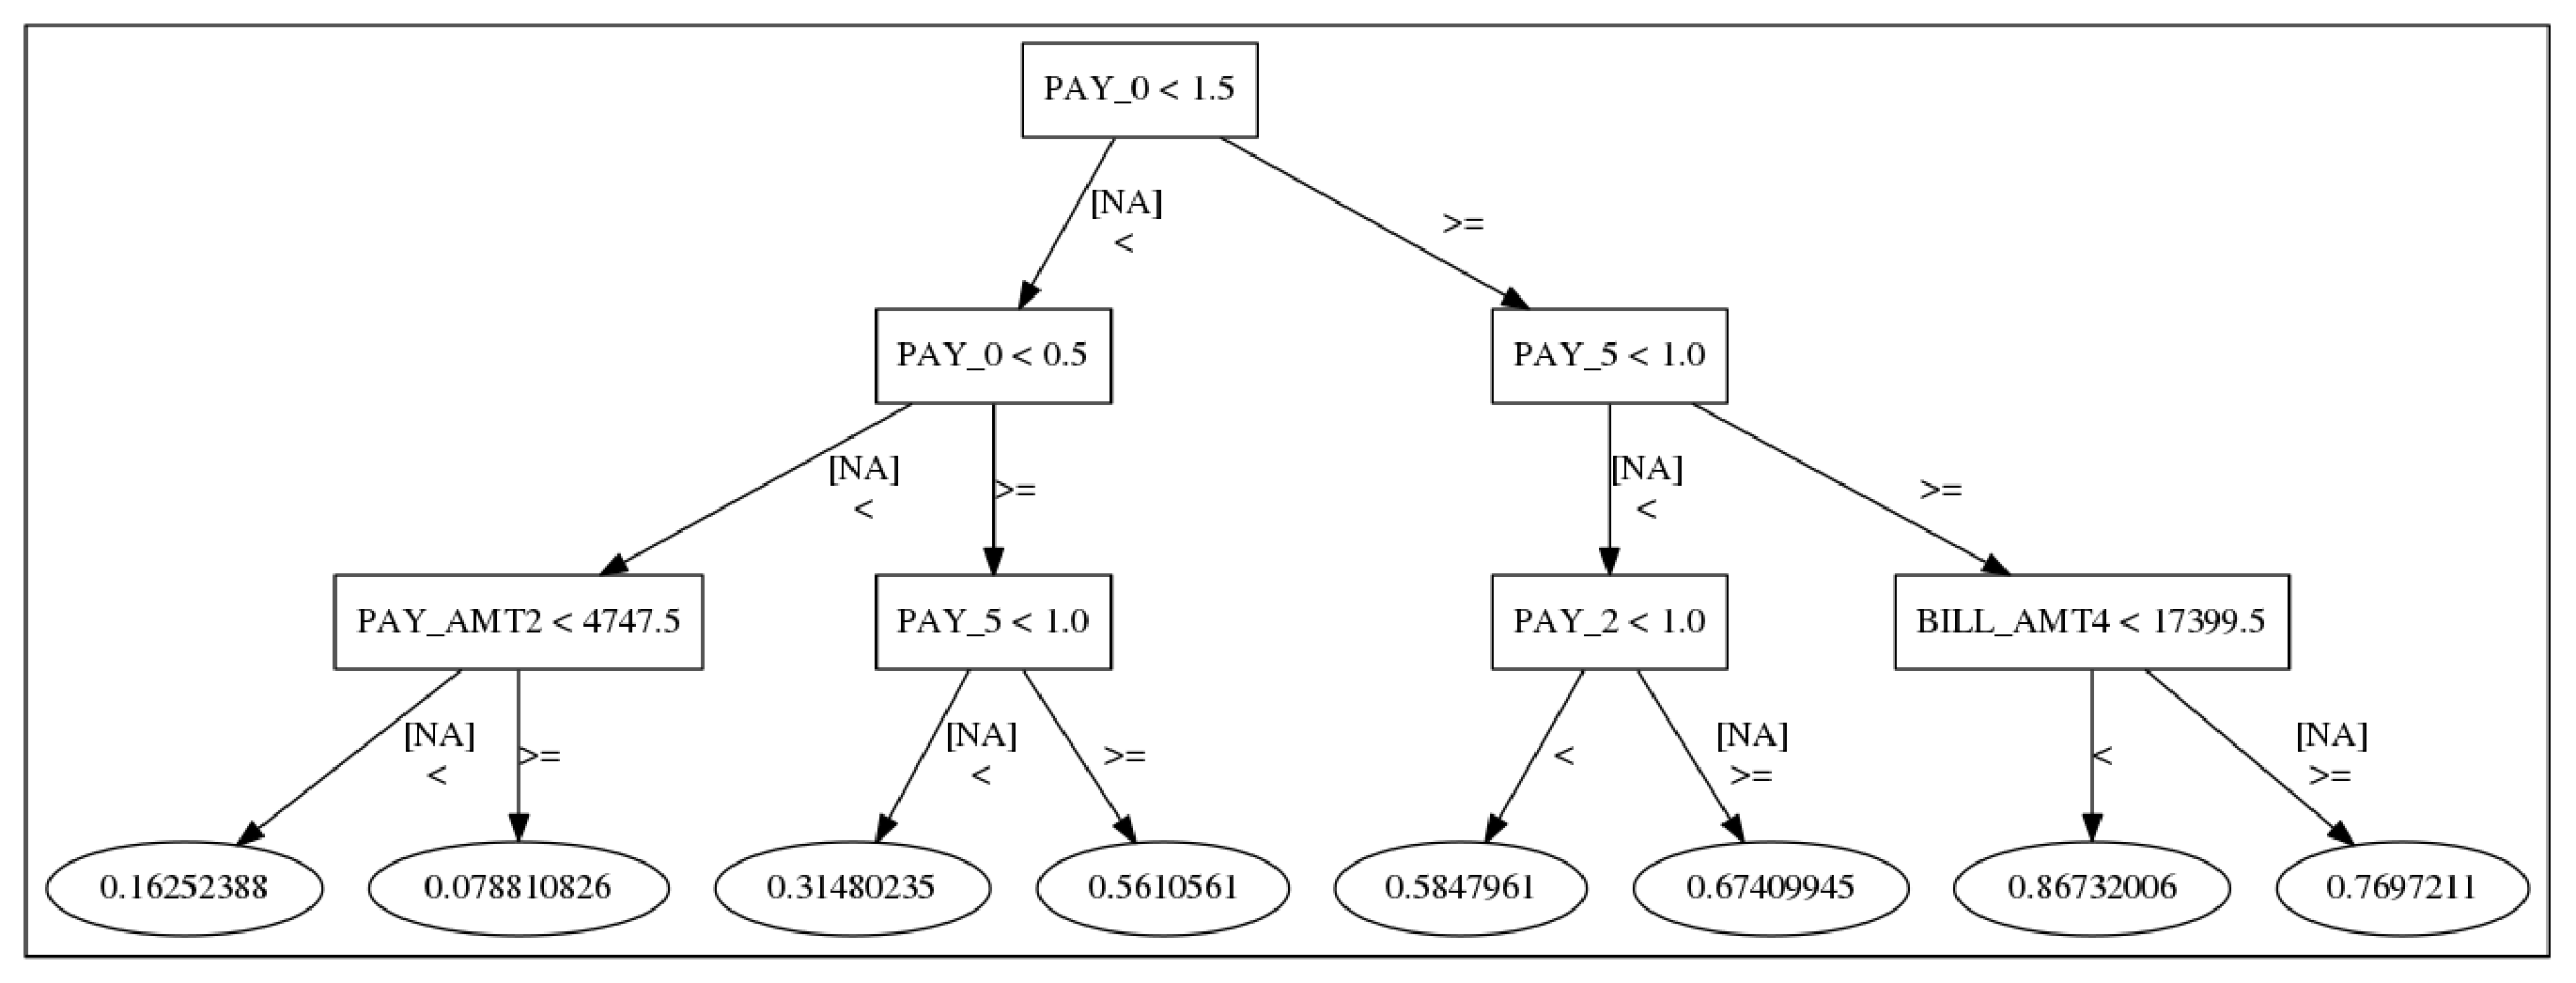
\includegraphics[scale=0.3]{img/figure_9.eps}
		\caption{$h_{\text{tree}}$ for $g_{\text{mono}}$ in a 30\% validation set randomly sampled from the UCI credit card dataset. An image of a depth-five $h_{\text{tree}}$ directed graph is available in the supplementary materials described in Section \ref{sec:software}.}
		\label{fig:cc_dt_surrogate}
	\end{center}
\end{figure*}

To continue explaining $g_{\text{mono}}$, a simple depth-three $h_{\text{tree}}$ model is trained to represent  $g_{\text{mono}}(\mathbf{X})$ in the validation set. $h_{\text{tree}}$ is displayed in Figure \ref{fig:cc_dt_surrogate}. $h_{\text{tree}}$ has a mean $R^2$ across three random folds in the validation set of 0.86 with a standard deviation of 0.0011 and a mean RMSE across the same folds of 0.08 with a standard deviation of 0.0003, indicating $h_{\text{tree}}$ is likely accurate and stable enough to be a helpful explanatory tool. The global importance of \texttt{PAY\_0} and the increase in $g_{\text{mono}}(\mathbf{x})$ associated with \texttt{PAY\_0 = 2} is reflected in the simple $h_{\text{tree}}$ model, along with several potentially important interactions between input features. For instance the lowest predicted probabilities from $h_{\text{tree}}$ occur when a customer's  most recent repayment status, \texttt{PAY\_0}, is less than 0.5 and their second most recent payment amount, \texttt{PAY\_AMT2}, is greater than or equal to NT\$ 4747.5. The highest predicted probabilities from $h_{\text{tree}}$ occur when \texttt{PAY\_0} $\geq$ \texttt{1.5}, a customers fifth most recent repayment status, \texttt{PAY\_5}, is 1 or more months late, and when a customer's fourth most recent bill amount, \texttt{BILL\_AMT4} is less than NT\$ 17399.5. In this simple depth-three $h_{\text{tree}}$ model, it appears that an interaction between \texttt{PAY\_0} and \texttt{PAY\_AMT2} may be leading to the very low probability of default predictions displayed in Figure \ref{fig:cc_pdp_ice}, while interactions between \texttt{PAY\_0}, \texttt{PAY\_5}, and \texttt{BILL\_AMT4} are potentially associated with the highest predicted probabilities. A more complex and accurate depth-five $h_{\text{tree}}$ model is available in the supplemental materials described in Section \ref{sec:software} and it presents greater detail regarding the interactions and decision paths that could lead to the modeled behavior for the lowest and highest probability of default customers. 
 
\begin{figure*}[htb]
	\begin{center}
		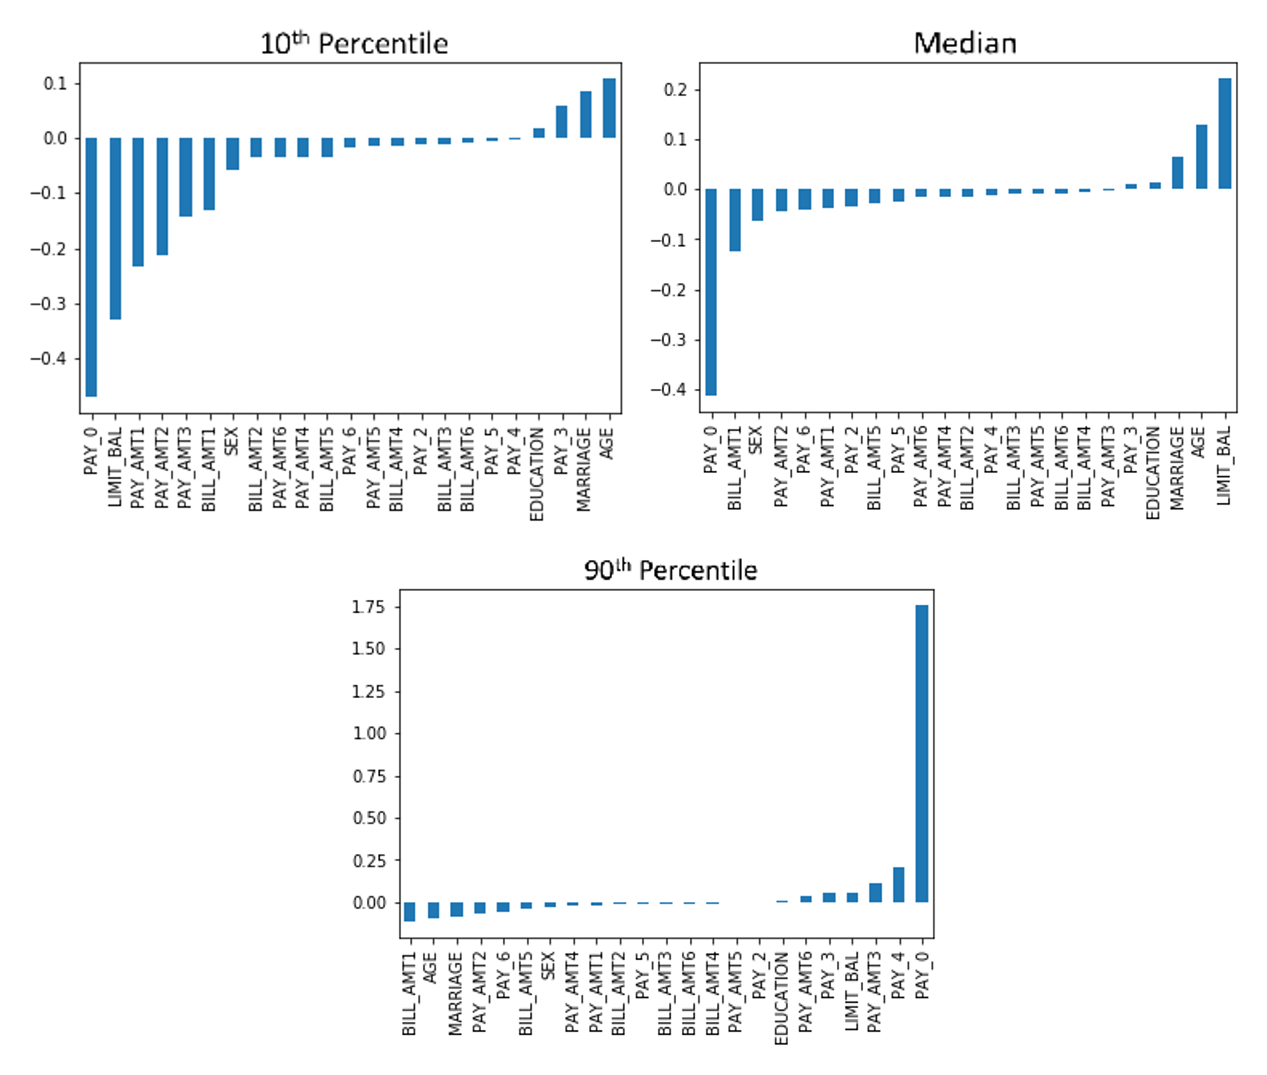
\includegraphics[scale=0.6]{img/figure_10.eps}
		\caption{Complete, consistent local feature contributions found using tree shap at three percentiles of $g_{\text{mono}}(\mathbf{X})$ in a 30\% validation set randomly sampled from the UCI credit card dataset.}
		\label{fig:cc_shap}
	\end{center}
\end{figure*}

Figure \ref{fig:cc_shap} displays local Shapley explanation values for three customers at the 10\textsuperscript{th}, median, and 90\textsuperscript{th} percentiles of $g_{\text{mono}}(\mathbf{X})$ in the validation set. The plots in Figure \ref{fig:cc_shap} are representative of the local Shapley explanations that could be generated for any $g_{\text{mono}}(\mathbf{x}), \mathbf{x} \in \mathcal{X}$. The values presented in Figure \ref{fig:cc_shap} are aligned with the general expectation that Shapley contributions will increase for increasing values of $g_{\text{mono}}(\mathbf{x})$. Reason codes to justify decisions based on $g_{\text{mono}}(\mathbf{x})$ predictions can also be generated for arbitrary $g_{\text{mono}}(\mathbf{x}), \mathbf{x} \in \mathcal{X}$ using local Shapley explanation values and the values of input features in $\mathbf{x}$. For the customer at the 90\textsuperscript{th} percentile of $g_{\text{mono}}(\mathbf{X})$ the likely top three reason codes to justify declining further credit are:

\begin{itemize}

\item Most recent payment is 2 months delayed.
\item Fourth most recent payment is 2 months delayed.
\item Third most recent payment amount is NT\$ 0.

\end{itemize} 

Analysis for an operational, mission-critical machine learning model would likely involve further investigation of partial dependence and ICE plots and perhaps deeper analysis of $h_{\text{tree}}$ models following Hu et al \cite{lime-sup}. Analysis would also probably continue on to diagnostic, or \textit{model debugging}, and fairness techniques such as:

\begin{itemize}

\item \textbf{Disparate impact analysis}: to uncover any unfairness in model predictions or errors across demographic segments.
\item \textbf{Residual analysis}: to check the fundamental assumptions of the model against relevant data partitions and to investigate outliers or observations exerting undue influence on $g(\mathbf{X})$. 
\item \textbf{Sensitivity analysis}: to explicitly test the trustworthiness of model predictions on simulated out-of-domain data or in other simulated scenarios of interest.  

\end{itemize} 

\noindent A successful explanatory and diagnostic analysis must also include remediating any discovered issues and documenting all findings. Examples of more detailed analyses along with the URLs to the data and software used to generate Figures \ref{fig:cc_global_shapley} -- \ref{fig:cc_shap} are available in Section \ref{sec:software}.

%-------------------------------------------------------------------------------
\section{Suggested Reading} \label{sec:suggested}
%-------------------------------------------------------------------------------

As stated in the introduction, this text focuses on a fairly narrow but practical sub-discipline of machine learning interpretability. As interpretability truly is a diverse subject with many other practically useful areas of study, additional subjects are suggested for further reading.

\subsection{White-box Models}

The application of post-hoc explanatory techniques is convenient for previously existing machine learning models, workflows, or pipelines. However, a more direct approach may be to train an interpretable white-box machine learning model which may or may not require additional post-hoc explanatory analysis. Monotonic XGBoost is an excellent option to evaluate because the software is open source, readily available, easily installable and deployable, and highly scalable \cite{xgboost}. Acclaimed work by the Rudin group at Duke University is also likely of interest to many users. They have developed several types of rule-based models \cite{corels}, \cite{sbrl}, linear model variants \cite{slim}, and many other novel algorithms suitable for use in high stakes, mission-critical prediction and decision-making scenarios. 

\subsection{Explainable Neural Networks (xNNs)}

Often considered the least transparent of black-box models, recent work in xNN implementation and explaining artificial neural network (ANN) predictions may render that notion of ANNs obsolete. Many of the breakthroughs in ANN explanation stem from the straightforward calculation of accurate derivatives of the trained ANN response function w.r.t. to input features made possible by the proliferation of deep learning toolkits such as tensorflow \cite{raissi2017physics}. These derivatives allow for the disaggregation of the trained ANN response function prediction, $g_{ANN}(\mathbf{X})$, into input feature contributions for any observation in the domain of $\mathcal{X}$. Popular techniques have names like DeepLIFT and integrated gradients \cite{deeplift}, \cite{integrated_grads}, \cite{grad_attr}. Explaining ANN predictions is impactful for at least two major reasons. While most users will be familiar with the wide-spread use of ANNs in pattern recognition, they are also used for more traditional data mining applications such as fraud detection, and even for regulated applications such as credit scoring \cite{mli_booklet}. Moreover, ANNs can now be used as accurate and explainable surrogate models, potentially increasing the fidelity of both global and local surrogate model techniques. For an excellent discussion of xNNs in a practical setting see \textit{Explainable Neural Networks based on Additive Index Models} by the Wells Fargo Corporate Model Risk group \cite{wf_xnn}.

\subsection{Fairness}

Fairness is yet another important facet of interpretability, and an admirable goal for any machine learning project whose outcomes will affect human lives. Traditional checks for fairness include assessing the average prediction, accuracy, and error across demographic segments. Today the study of fairness in machine learning is widening and progressing rapidly. Users who would like to stay abreast of developments in the fairness space should follow the free online book by leading researchers, \textit{Fairness and Machine Learning} \cite{fairness_book}. The book's website currently includes references to other fairness materials. Users may also be interested in the broader organization for fairness, accountability, and transparency in machine learning or FATML. FATML maintains a list of pertinent scholarship on their website: \url{https://www.fatml.org/}. 

\subsection{Model Debugging}

As alluded to in previous sections, the techniques in this text enable practitioners to \textit{explain} and hopefully understand complex models. Trust is a related and somewhat orthogonal concept in interpretability, because models can certainly be explained and not trusted, and conversely, be trusted and not explainable. The growing field of model debugging empowers users to trust their complex model predictions and to diagnose and treat any discovered undesirable behaviors. While residual and sensitivity analysis typically play a role in model debugging exercises, readers are encouraged to investigate newer methods such as \textit{anchors} and burgeoning work in adversarial examples \cite{anchors}, \cite{adversarial_sameer}. 
 
%-------------------------------------------------------------------------------
\section{Supplementary Materials and Software Resources } \label{sec:software}
%-------------------------------------------------------------------------------

To make the discussed results useful and reproducible for practitioners, several online supporting materials and software resources are freely available. 

\begin{itemize}

	\item Supplementary materials and any corrections or updates to this text are available  at: \url{https://github.com/jphall663/jsm_2018_paper}.

	\item Simulated data experiments, including experiments on random data, and the UCI credit card dataset use case are available at: \url{https://github.com/h2oai/mli-resources/tree/master/lime_shap_treeint_compare}. General instructions for using these resources, including a Dockerfile which builds the complete runtime environment with all dependencies, are available here: \url{https://github.com/h2oai/mli-resources}.

	\item In-depth example explanatory use cases for the UCI credit card dataset are available at: \url{https://github.com/jphall663/interpretable_machine_learning_with_python}.

	\item A curated list of interpretability software is available at: \url{https://github.com/jphall663/awesome-machine-learning-interpretability}.

\end{itemize}

%-------------------------------------------------------------------------------
\section{Acknowledgements} 
%-------------------------------------------------------------------------------

The author wishes to thank Sri Ambati, Arno Candel, Mark Chan,  Doug Deloy, Lauren DiPerna, Mateusz Dymczyk, Navdeep Gill, Megan and Michal Kurka, Lingyao Meng, Mattias M\"uller, Wen Phan and other makers past and present at H2O.ai who turned explainability into a software application and learned the lessons discussed in this text along with me. The author thanks Leland Wilkinson at H2O.ai and the University of Illinois at Chicago (UIC) for his continued mentorship and guidance. 

%-------------------------------------------------------------------------------
%\section{References}
%-------------------------------------------------------------------------------

\bibliographystyle{plain}
\bibliography{jsm_2018_paper}

\end{document}


